\documentclass[../main/Notes.tex]{subfiles}
\begin{document}

\section[Measuring Beliefs II]{Measuring Beliefs II \iftoggle{showdates}{\small{\textit{2014-05-09}}}{}}

\subsection{Probabilities of Continuous Random Variables}\index{Continuous Random Variable}
How tall is Frank Jäkel? 1.80m, 1.70m, 1.68m, 1.69m, or even 1.7034241m?

Not only are there problems with real numbers like 1.7034241, but also with the question the Bayesian view inevitably asks: ``What do you think is the probability for that size?''

One sees: continuous random variables are difficult. There is an infinite uncountable range of numbers and one shall assign probabilities for them. This leads straight to the question: ``What's the probability of a real number?''

In the following section this problem gets tackled in three ways.

\subsubsection[Probability Density Function (PDF)]{Solution 1: Histograms (Probability Density Function, PDF)}\index{PDF}
The first and naive way is to discretize the sample space $\mathbb{R}$ into bins and assign probabilities to those bins (figure \ref{fig:2014-05-09_Histogram}).

\begin{figure}[!ht]
\centering
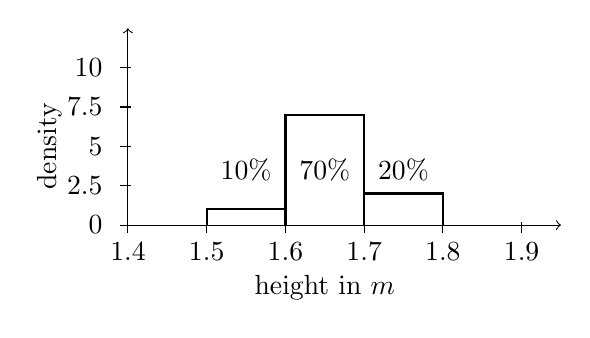
\begin{tikzpicture}

  % horizontal axis
  \draw[->] (0, 0) -- (5.5, 0);
  % ticks horizontal
  \foreach \x in {0,...,5}
    \draw (\x,1pt) -- (\x,-3pt);
  % labels horizontal
  \draw	(0,-0.1) node[anchor=north] {1.4}
		    (1,-0.1) node[anchor=north] {1.5}
		    (2,-0.1) node[anchor=north] {1.6}
		    (3,-0.1) node[anchor=north] {1.7}
		    (4,-0.1) node[anchor=north] {1.8}
		    (5,-0.1) node[anchor=north] {1.9}
        ;
  % axis label
  \draw (2.5,-0.8) node {height in $m$};
  
  % vertical axis
  \draw[->] (0, 0) -- (0, 2.5);
  % ticks vertical
  \foreach \y in {0,0.5,1,1.5,2}
    \draw (1pt, \y) -- (-3pt, \y);
  % labels vertical
  \draw (-0.2,0.0) node[anchor=east]  {0}
        (-0.2,0.5) node[anchor=east]  {2.5}
        (-0.2,1.0) node[anchor=east]  {5}
        (-0.2,1.5) node[anchor=east]  {7.5}
        (-0.2,2.0) node[anchor=east] {10}
        ;
  % axis label
  \draw (-1,1) node[rotate=90] {density};
  
  % first box
  \draw[thick] (1, 0) -- (1, 0.2) -- (2, 0.2) -- (2, 0);
  % second box
  \draw[thick] (2, 0) -- (2, 1.4) -- (3, 1.4) -- (3, 0);
  % third box
  \draw[thick] (3, 0) -- (3, 0.4) -- (4, 0.4) -- (4, 0);
  
  % box labels
  \draw (1.5, 0.7) node{$10 \%$};
  \draw (2.5, 0.7) node{$70 \%$};
  \draw (3.5, 0.7) node{$20 \%$};
  
\end{tikzpicture}
\caption{Histogram}
\label{fig:2014-05-09_Histogram}
\end{figure}

Note that \textbf{the area describes the probability}. For the second box, one would assign a y-value of 7, such that the width (0.1) times the height equals the probability ($0.1\cdot 7 = 0.7$).

For a finer granularity one can now change the resolution of the bins and split the probabilities among them (figure \ref{fig:2014-05-09_fineHistogram}.

\begin{figure}[!ht]
\centering
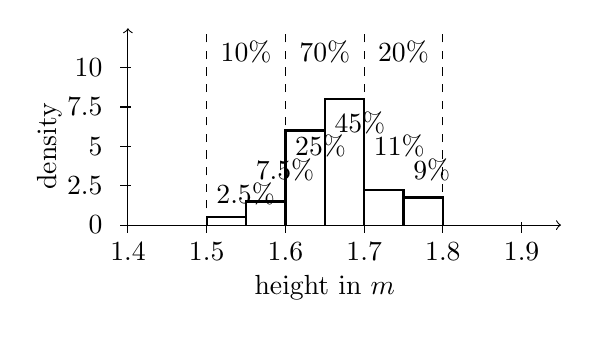
\begin{tikzpicture}

  % horizontal axis
  \draw[->] (0, 0) -- (5.5, 0);
  % ticks horizontal
  \foreach \x in {0,...,5}
    \draw (\x,1pt) -- (\x,-3pt);
  % labels horizontal
  \draw	(0,-0.1) node[anchor=north] {1.4}
		    (1,-0.1) node[anchor=north] {1.5}
		    (2,-0.1) node[anchor=north] {1.6}
		    (3,-0.1) node[anchor=north] {1.7}
		    (4,-0.1) node[anchor=north] {1.8}
		    (5,-0.1) node[anchor=north] {1.9}
        ;
  % axis label
  \draw (2.5,-0.8) node {height in $m$};
  
  % vertical axis
  \draw[->] (0, 0) -- (0, 2.5);
  % ticks vertical
  \foreach \y in {0,0.5,1,1.5,2}
    \draw (1pt, \y) -- (-3pt, \y);
  % labels vertical
  \draw (-0.2,0.0) node[anchor=east]  {0}
        (-0.2,0.5) node[anchor=east]  {2.5}
        (-0.2,1.0) node[anchor=east]  {5}
        (-0.2,1.5) node[anchor=east]  {7.5}
        (-0.2,2.0) node[anchor=east] {10}
        ;
  % axis label
  \draw (-1,1) node[rotate=90] {density};
  
  % first box
  \draw[thick] (1.0, 0) -- (1.0, 0.1) -- (1.5, 0.1) -- (1.5, 0);
  \draw[thick] (1.5, 0) -- (1.5, 0.3) -- (2.0, 0.3) -- (2.0, 0);
  % second box
  \draw[thick] (2.0, 0) -- (2.0, 1.2) -- (2.5, 1.2) -- (2.5, 0);
  \draw[thick] (2.5, 0) -- (2.5, 1.6) -- (3.0, 1.6) -- (3.0, 0);
  % third box
  \draw[thick] (3.0, 0) -- (3.0, 0.45) -- (3.5, 0.45) -- (3.5, 0);
  \draw[thick] (3.5, 0) -- (3.5, 0.35) -- (4.0, 0.35) -- (4.0, 0);
  
  % box labels
  \draw (1.5, 2.2) node{$10 \%$};
  \draw (2.5, 2.2) node{$70 \%$};
  \draw (3.5, 2.2) node{$20 \%$};
  
  \draw (1.0, 0.4) node[anchor=west]{$2.5 \%$};
  \draw (1.5, 0.7) node[anchor=west]{$7.5 \%$};
  \draw (2.0, 1.0) node[anchor=west]{$25 \%$};
  \draw (2.5, 1.3) node[anchor=west]{$45 \%$};
  \draw (3.0, 1.0) node[anchor=west]{$11 \%$};
  \draw (3.5, 0.7) node[anchor=west]{$ 9 \%$};
  
  % vertical separation lines
  \draw[thin, dashed] (1, 0) -- (1, 2.5);
  \draw[thin, dashed] (2, 0) -- (2, 2.5);
  \draw[thin, dashed] (3, 0) -- (3, 2.5);
  \draw[thin, dashed] (4, 0) -- (4, 2.5);
  
\end{tikzpicture}
\caption{Histogram with higher resolution}
\label{fig:2014-05-09_fineHistogram}
\end{figure}

\begin{samepage}
\textbf{Extreme cases}
Usually this will yield a nice distribution of how beliefs are. However, there are two special extreme cases.

\begin{enumerate}
  \item[] The first case is that all values are equally probable: Since we have infinitely many values on the real number line, the probability for each individual value is $\frac{1}{n} \Rightarrow \lim\limits_{n\rightarrow\infty} \frac{1}{n} = 0$. 
  \item[] The second case is that the full probability gets assigned to one single value. Since a single value has the width 0, again the probability will become 0 for all values.
\end{enumerate}
\end{samepage}

\textbf{The probability density function}
However, if the resulting histogram is somewhere between those extreme cases, then the limit of the distribution yields the probability density function (figure \ref{fig:2014-05-09_pdf}).

\begin{figure}[!ht]
\centering
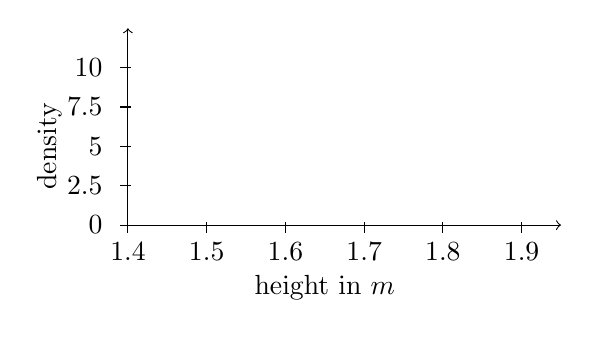
\begin{tikzpicture}
  
  % horizontal axis
  \draw[->] (0, 0) -- (5.5, 0);
  % ticks horizontal
  \foreach \x in {0,...,5}
    \draw (\x,1pt) -- (\x,-3pt);
  % labels horizontal
  \draw	(0,-0.1) node[anchor=north] {1.4}
		    (1,-0.1) node[anchor=north] {1.5}
		    (2,-0.1) node[anchor=north] {1.6}
		    (3,-0.1) node[anchor=north] {1.7}
		    (4,-0.1) node[anchor=north] {1.8}
		    (5,-0.1) node[anchor=north] {1.9}
        ;
  % axis label
  \draw (2.5,-0.8) node {height in $m$};
  
  % vertical axis
  \draw[->] (0, 0) -- (0, 2.5);
  % ticks vertical
  \foreach \y in {0,0.5,1,1.5,2}
    \draw (1pt, \y) -- (-3pt, \y);
  % labels vertical
  \draw (-0.2,0.0) node[anchor=east]  {0}
        (-0.2,0.5) node[anchor=east]  {2.5}
        (-0.2,1.0) node[anchor=east]  {5}
        (-0.2,1.5) node[anchor=east]  {7.5}
        (-0.2,2.0) node[anchor=east] {10}
        ;
  % axis label
  \draw (-1,1) node[rotate=90] {density};
  
  \draw[thick] plot[smooth] file {../data/2014-05-09_HistogramToPDF.txt};
\end{tikzpicture}
\caption{Probability density function}
\label{fig:2014-05-09_pdf}
\end{figure}

As mentioned before it's still not possible to calculate the probability of a specific number. What is possible though, is calculating the probability of an interval. This is useful, since people always bet on intervals. For instance, betting on ``2'' means to bet on the interval $\left[2,3\right[$.

\subsubsection[Cumulative Density Function (CDF)]{Solution 2: Cumulative Density Function, CDF}\index{CDF}
To calculate the probability of an interval it's possible to simply sum up all probabilities in the specific interval.

This can be done by integration of the PDF\index{PDF} (see figure \ref{fig:2014-05-09_pdf_to_cdf}).

\begin{figure}[!ht]
\centering
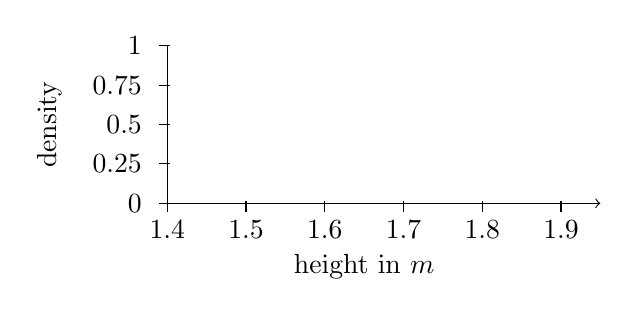
\begin{tikzpicture}
  
  % horizontal axis
  \draw[->] (0, 0) -- (5.5, 0);
  % ticks horizontal
  \foreach \x in {0,...,5}
    \draw (\x,1pt) -- (\x,-3pt);
  % labels horizontal
  \draw	(0,-0.1) node[anchor=north] {1.4}
		    (1,-0.1) node[anchor=north] {1.5}
		    (2,-0.1) node[anchor=north] {1.6}
		    (3,-0.1) node[anchor=north] {1.7}
		    (4,-0.1) node[anchor=north] {1.8}
		    (5,-0.1) node[anchor=north] {1.9}
        ;
  % axis label
  \draw (2.5,-0.8) node {height in $m$};
  
  % vertical axis
  \draw[-] (0, 0) -- (0, 2);
  % ticks vertical
  \foreach \y in {0,0.5,1,1.5,2}
    \draw (1pt, \y) -- (-3pt, \y);
  % labels vertical
  \draw (-0.2,0.0) node[anchor=east] {0}
        (-0.2,0.5) node[anchor=east] {0.25}
        (-0.2,1.0) node[anchor=east] {0.5}
        (-0.2,1.5) node[anchor=east] {0.75}
        (-0.2,2.0) node[anchor=east] {1}
        ;
  % axis label
  \draw (-1.5,1) node[rotate=90] {density};
  
  \draw[thick] plot[smooth] file {../data/2014-05-09_CDF.txt};
\end{tikzpicture}
\caption{Cumulative density function}
\label{fig:2014-05-09_pdf_to_cdf}
\end{figure}


\subsubsection[Parametric Gaussian Distribution]{Solution 3: Parametric Distribution}\index{Parametric Distribution}
The only remaining problem is deriving the correct probability density function. We can avoid this by using a very common statistics method and model the PDF\index{PDF} as a Gaussian distribution\index{Gaussian Distribution}.

This way we reduce the problem finding the correct function to finding the correct parameters.

\bigskip

The Gaussian distribution (see figure \ref{fig:2014-05-09-diffGaussDistr}) is defined as
\begin{align*}
p(X=x) = \frac{1}{2\pi\sigma^2}e^{-\frac{1}{2}\left(\frac{\mu-x}{\sigma}\right)^2} &= \phi(x;\mu,\sigma) = \phi\left(\frac{\mu-x}{\sigma};0,1\right) \\
\frac{\mu-x}{\sigma}&=z
\end{align*}

The corresponding integral is $\Phi$ (see figure \ref{fig:2014-05-09-diffGaussDistr}).
\begin{align*}
P(X \leq t) = \int\limits_{-\infty}^{t}{p(X=x)} dx &= \Phi(t;\mu,\sigma)
\end{align*}

\begin{figure}[!ht]
\centering
\begin{tikzpicture}
  \begin{axis}[every axis plot post/.append style={mark=none, domain=-4:4, samples=50, smooth}, 
    axis x line*=bottom, axis y line*=left, enlargelimits=upper, name=gauss]
    \addplot [red]    {gauss(0,0.5)};% node[pos=0.4,  anchor=east] {$\sigma=0.5$};
      \addlegendentry{$\mu=0,\sigma=0.5$}
    \addplot [green]  {gauss(0,1)};%   node[pos=0.6,  anchor=west] {$\sigma=1$};
      \addlegendentry{$\mu=0,\sigma=1$}
    \addplot [blue]   {gauss(0,2)};%   node[pos=0.85, anchor=west] {$\sigma=2$};
      \addlegendentry{$\mu=0,\sigma=2$}
    \addplot [yellow] {gauss(1,1)};%   node[pos=0.7,  anchor=west] {$\mu=1,\sigma=1$};
      \addlegendentry{$\mu=1,\sigma=1$}
  \end{axis}

  \begin{axis}[every axis plot post/.append style={mark=none, domain=-4:4, samples=50, smooth}, legend style={at={(0.98,0.02)}, anchor=south east}, 
    axis x line*=bottom, axis y line*=left, enlargelimits=upper, name=Gauss, at=(gauss.right of east), anchor=left of west]
    \addplot [red]    {Gauss(0,0.5)};% node[pos=0.5,  anchor=west] {$\sigma=0.5$};
      \addlegendentry{$\mu=0,\sigma=0.5$}
    \addplot [green]  {Gauss(0,1)};%   node[pos=0.5,  anchor=east] {$\sigma=1$};
      \addlegendentry{$\mu=0,\sigma=1$}
    \addplot [blue]   {Gauss(0,2)};%   node[pos=0.85, anchor=west] {$\sigma=2$};
      \addlegendentry{$\mu=0,\sigma=1$}
    \addplot [yellow] {Gauss(1,1)};%   node[pos=0.7,  anchor=west] {$\mu=1,\sigma=1$};
      \addlegendentry{$\mu=1,\sigma=1$}
  \end{axis}
\end{tikzpicture}
\caption{Left: Gaussian distributions. Right: Their corresponding integrals. Parameters: $\mu=0$ and $\sigma = 0.5, 1, 2$, and $\mu=1, \sigma=1$.}
\label{fig:2014-05-09-diffGaussDistr}
\end{figure}

The area of the standard deviation\index{Standard Deviation} ($\mu - \sigma \leq X \leq \mu + \sigma$) has a probability of approximately 68 \% (see figure \ref{fig:2014-05-09-std}).
\begin{align*}
P(\mu - \sigma \leq X \leq \mu + \sigma) = \Phi(\mu+\sigma;\mu,\sigma) - \Phi(\mu-\sigma;\mu,\sigma) \approx 68 \%
\end{align*}

\begin{figure}[!ht]
\centering
\begin{tikzpicture}
\begin{axis}[axis x line*=bottom, axis y line*=left, enlargelimits=upper, axis on top, domain=-4:4, y post scale=0.5]
  \addplot+[domain=-1:1, samples=100, pattern=flexible hatch, mark=none
            hatch distance=5pt, hatch thickness=0.5pt,
            draw=green, pattern color=green!40, area legend]
            {gauss(0,1)} \closedcycle;
    \addlegendentry{$\approx 68\%$}
  \addplot[color=red, samples=50, smooth] {gauss(0,1)};
    \addlegendentry{$\mu=0,\sigma=1$}
\end{axis}
\end{tikzpicture}
\caption{The area of the standard deviation yields approximately 68 \%}
\label{fig:2014-05-09-std}
\end{figure}

\begin{samepage}
We can also find other useful probabilities which are commonly used to do statistics:
\begin{itemize}
	\item $\mu \pm \sigma \approx 68\%$
	\item $\mu \pm 2\sigma \approx 95\%$
	\item $\mu \pm 3\sigma \approx 99\%$
\end{itemize}
\end{samepage}


\subsection{Proper Scoring Rules}\index{Proper Scoring Rule}
Multiple choice tests would be better if you would state ``how your belief is, that this is right'', rather than just answering the question (For more about this see page \pageref{ex4_4_solution}).

\bigskip

Take a look at this example: \\ \textit{The EU population is bigger than the US population. \\
Give the belief for this to be true. \\(This means 0 = ``I believe this is false'', 1 = ``I believe this is true'', 0.5 = ``I don't know'')}

\bigskip

The aim of a proper scoring rule is to yield a high gain if the answer is true and the belief in it is high, but yield no gain if the answer is false but the belief in it high.

$q$ is the belief assigned to the answer given, $X$ is 1 if the statement was true or 0 if it was false.
\begin{align*}
L\left(X,q\right) &= \left(X-q\right)^2 \\
                  &= X^2-2qX+q^2 \mbox{ \textit{(note: $X^2 = X$, since only 0 or 1)}} \\
                  &= X\left(1-2q\right)+q^2
\end{align*}

\subsubsection*{Penalty for lying}
\begin{align*}
E\left(L\left(X,q\right)\right) &= p-2pq+q^2 = \left(p-p^2\right) + \left(p^2-2pq+q^2\right) \\&= \underbrace{p\left(1-p\right)}_\text{basic loss} + \underbrace{\left(p-q\right)^2}_\text{penalty for lying}
\end{align*}

\subsubsection*{How to answer?}
If one's belief is p, which q will yield the best gain (i.e. will minimize the expected loss)?

To answer this the expected loss\index{Expected Loss} function can be minimized, i.e. one can search the first derivative and set it to zero. 

\begin{align*}
E\left(L\left(p,q\right)\right) &= p\left(1-2q\right)+q^2 \\
\frac{\partial E\left(L\left(p,q\right)\right)}{\partial q} &= -2p + 2q \\
\rightarrow 0 &= -2p + 2q \\
\Leftrightarrow p &= q
\end{align*}

As can be seen the loss function is minimal if $p=q$, i.e. if the person answering is telling the truth.

\end{document}